% Options for packages loaded elsewhere
\PassOptionsToPackage{unicode}{hyperref}
\PassOptionsToPackage{hyphens}{url}
\PassOptionsToPackage{dvipsnames,svgnames,x11names}{xcolor}
%
\documentclass[
]{article}

\usepackage{amsmath,amssymb}
\usepackage{lmodern}
\usepackage{iftex}
\ifPDFTeX
  \usepackage[T1]{fontenc}
  \usepackage[utf8]{inputenc}
  \usepackage{textcomp} % provide euro and other symbols
\else % if luatex or xetex
  \usepackage{unicode-math}
  \defaultfontfeatures{Scale=MatchLowercase}
  \defaultfontfeatures[\rmfamily]{Ligatures=TeX,Scale=1}
\fi
% Use upquote if available, for straight quotes in verbatim environments
\IfFileExists{upquote.sty}{\usepackage{upquote}}{}
\IfFileExists{microtype.sty}{% use microtype if available
  \usepackage[]{microtype}
  \UseMicrotypeSet[protrusion]{basicmath} % disable protrusion for tt fonts
}{}
\makeatletter
\@ifundefined{KOMAClassName}{% if non-KOMA class
  \IfFileExists{parskip.sty}{%
    \usepackage{parskip}
  }{% else
    \setlength{\parindent}{0pt}
    \setlength{\parskip}{6pt plus 2pt minus 1pt}}
}{% if KOMA class
  \KOMAoptions{parskip=half}}
\makeatother
\usepackage{xcolor}
\setlength{\emergencystretch}{3em} % prevent overfull lines
\setcounter{secnumdepth}{-\maxdimen} % remove section numbering
% Make \paragraph and \subparagraph free-standing
\ifx\paragraph\undefined\else
  \let\oldparagraph\paragraph
  \renewcommand{\paragraph}[1]{\oldparagraph{#1}\mbox{}}
\fi
\ifx\subparagraph\undefined\else
  \let\oldsubparagraph\subparagraph
  \renewcommand{\subparagraph}[1]{\oldsubparagraph{#1}\mbox{}}
\fi

\usepackage{color}
\usepackage{fancyvrb}
\newcommand{\VerbBar}{|}
\newcommand{\VERB}{\Verb[commandchars=\\\{\}]}
\DefineVerbatimEnvironment{Highlighting}{Verbatim}{commandchars=\\\{\}}
% Add ',fontsize=\small' for more characters per line
\usepackage{framed}
\definecolor{shadecolor}{RGB}{241,243,245}
\newenvironment{Shaded}{\begin{snugshade}}{\end{snugshade}}
\newcommand{\AlertTok}[1]{\textcolor[rgb]{0.68,0.00,0.00}{#1}}
\newcommand{\AnnotationTok}[1]{\textcolor[rgb]{0.37,0.37,0.37}{#1}}
\newcommand{\AttributeTok}[1]{\textcolor[rgb]{0.40,0.45,0.13}{#1}}
\newcommand{\BaseNTok}[1]{\textcolor[rgb]{0.68,0.00,0.00}{#1}}
\newcommand{\BuiltInTok}[1]{\textcolor[rgb]{0.00,0.23,0.31}{#1}}
\newcommand{\CharTok}[1]{\textcolor[rgb]{0.13,0.47,0.30}{#1}}
\newcommand{\CommentTok}[1]{\textcolor[rgb]{0.37,0.37,0.37}{#1}}
\newcommand{\CommentVarTok}[1]{\textcolor[rgb]{0.37,0.37,0.37}{\textit{#1}}}
\newcommand{\ConstantTok}[1]{\textcolor[rgb]{0.56,0.35,0.01}{#1}}
\newcommand{\ControlFlowTok}[1]{\textcolor[rgb]{0.00,0.23,0.31}{#1}}
\newcommand{\DataTypeTok}[1]{\textcolor[rgb]{0.68,0.00,0.00}{#1}}
\newcommand{\DecValTok}[1]{\textcolor[rgb]{0.68,0.00,0.00}{#1}}
\newcommand{\DocumentationTok}[1]{\textcolor[rgb]{0.37,0.37,0.37}{\textit{#1}}}
\newcommand{\ErrorTok}[1]{\textcolor[rgb]{0.68,0.00,0.00}{#1}}
\newcommand{\ExtensionTok}[1]{\textcolor[rgb]{0.00,0.23,0.31}{#1}}
\newcommand{\FloatTok}[1]{\textcolor[rgb]{0.68,0.00,0.00}{#1}}
\newcommand{\FunctionTok}[1]{\textcolor[rgb]{0.28,0.35,0.67}{#1}}
\newcommand{\ImportTok}[1]{\textcolor[rgb]{0.00,0.46,0.62}{#1}}
\newcommand{\InformationTok}[1]{\textcolor[rgb]{0.37,0.37,0.37}{#1}}
\newcommand{\KeywordTok}[1]{\textcolor[rgb]{0.00,0.23,0.31}{#1}}
\newcommand{\NormalTok}[1]{\textcolor[rgb]{0.00,0.23,0.31}{#1}}
\newcommand{\OperatorTok}[1]{\textcolor[rgb]{0.37,0.37,0.37}{#1}}
\newcommand{\OtherTok}[1]{\textcolor[rgb]{0.00,0.23,0.31}{#1}}
\newcommand{\PreprocessorTok}[1]{\textcolor[rgb]{0.68,0.00,0.00}{#1}}
\newcommand{\RegionMarkerTok}[1]{\textcolor[rgb]{0.00,0.23,0.31}{#1}}
\newcommand{\SpecialCharTok}[1]{\textcolor[rgb]{0.37,0.37,0.37}{#1}}
\newcommand{\SpecialStringTok}[1]{\textcolor[rgb]{0.13,0.47,0.30}{#1}}
\newcommand{\StringTok}[1]{\textcolor[rgb]{0.13,0.47,0.30}{#1}}
\newcommand{\VariableTok}[1]{\textcolor[rgb]{0.07,0.07,0.07}{#1}}
\newcommand{\VerbatimStringTok}[1]{\textcolor[rgb]{0.13,0.47,0.30}{#1}}
\newcommand{\WarningTok}[1]{\textcolor[rgb]{0.37,0.37,0.37}{\textit{#1}}}

\providecommand{\tightlist}{%
  \setlength{\itemsep}{0pt}\setlength{\parskip}{0pt}}\usepackage{longtable,booktabs,array}
\usepackage{calc} % for calculating minipage widths
% Correct order of tables after \paragraph or \subparagraph
\usepackage{etoolbox}
\makeatletter
\patchcmd\longtable{\par}{\if@noskipsec\mbox{}\fi\par}{}{}
\makeatother
% Allow footnotes in longtable head/foot
\IfFileExists{footnotehyper.sty}{\usepackage{footnotehyper}}{\usepackage{footnote}}
\makesavenoteenv{longtable}
\usepackage{graphicx}
\makeatletter
\def\maxwidth{\ifdim\Gin@nat@width>\linewidth\linewidth\else\Gin@nat@width\fi}
\def\maxheight{\ifdim\Gin@nat@height>\textheight\textheight\else\Gin@nat@height\fi}
\makeatother
% Scale images if necessary, so that they will not overflow the page
% margins by default, and it is still possible to overwrite the defaults
% using explicit options in \includegraphics[width, height, ...]{}
\setkeys{Gin}{width=\maxwidth,height=\maxheight,keepaspectratio}
% Set default figure placement to htbp
\makeatletter
\def\fps@figure{htbp}
\makeatother

\makeatletter
\makeatother
\makeatletter
\makeatother
\makeatletter
\@ifpackageloaded{caption}{}{\usepackage{caption}}
\AtBeginDocument{%
\ifdefined\contentsname
  \renewcommand*\contentsname{Table of contents}
\else
  \newcommand\contentsname{Table of contents}
\fi
\ifdefined\listfigurename
  \renewcommand*\listfigurename{List of Figures}
\else
  \newcommand\listfigurename{List of Figures}
\fi
\ifdefined\listtablename
  \renewcommand*\listtablename{List of Tables}
\else
  \newcommand\listtablename{List of Tables}
\fi
\ifdefined\figurename
  \renewcommand*\figurename{Figure}
\else
  \newcommand\figurename{Figure}
\fi
\ifdefined\tablename
  \renewcommand*\tablename{Table}
\else
  \newcommand\tablename{Table}
\fi
}
\@ifpackageloaded{float}{}{\usepackage{float}}
\floatstyle{ruled}
\@ifundefined{c@chapter}{\newfloat{codelisting}{h}{lop}}{\newfloat{codelisting}{h}{lop}[chapter]}
\floatname{codelisting}{Listing}
\newcommand*\listoflistings{\listof{codelisting}{List of Listings}}
\makeatother
\makeatletter
\@ifpackageloaded{caption}{}{\usepackage{caption}}
\@ifpackageloaded{subcaption}{}{\usepackage{subcaption}}
\makeatother
\makeatletter
\@ifpackageloaded{tcolorbox}{}{\usepackage[many]{tcolorbox}}
\makeatother
\makeatletter
\@ifundefined{shadecolor}{\definecolor{shadecolor}{rgb}{.97, .97, .97}}
\makeatother
\makeatletter
\makeatother
\ifLuaTeX
  \usepackage{selnolig}  % disable illegal ligatures
\fi
\IfFileExists{bookmark.sty}{\usepackage{bookmark}}{\usepackage{hyperref}}
\IfFileExists{xurl.sty}{\usepackage{xurl}}{} % add URL line breaks if available
\urlstyle{same} % disable monospaced font for URLs
\hypersetup{
  pdftitle={Mission: Iconic Reefs and National Coral Reef Monitoring Program Benthic Analysis},
  pdfauthor={Nicole Krampitz, Julia Mateski, and Dione Swanson},
  colorlinks=true,
  linkcolor={blue},
  filecolor={Maroon},
  citecolor={Blue},
  urlcolor={Blue},
  pdfcreator={LaTeX via pandoc}}

\title{Mission: Iconic Reefs and National Coral Reef Monitoring Program
Benthic Analysis}
\author{Nicole Krampitz, Julia Mateski, and Dione Swanson}
\date{}

\begin{document}
\maketitle
\ifdefined\Shaded\renewenvironment{Shaded}{\begin{tcolorbox}[sharp corners, boxrule=0pt, interior hidden, borderline west={3pt}{0pt}{shadecolor}, enhanced, breakable, frame hidden]}{\end{tcolorbox}}\fi

The
\href{https://www.fisheries.noaa.gov/southeast/habitat-conservation/restoring-seven-iconic-reefs-mission-recover-coral-reefs-florida-keys}{Mission:
Iconic Reefs} (M:IR) project is a decades-long ambitious effort to
restore seven key coral reef areas in the Florida Keys National Marine
Sanctuary (FKNMS) via coral propagation and transplantation. Restoration
is being carried out in planned phases along with biennial monitoring to
provide a quantitative measure of restoration effects over time. The
primary goal of this monitoring is to compare fish populations, coral
populations, and benthic community metrics within M:IR restoration areas
to those reefs in the broader Florida Keys in partnership with the
National Coral Reef Monitoring Program (NCRMP). Currently, two rounds of
surveying have been completed (in 2022 and 2024) to establish baseline
conditions. This report focuses on coral populations and benthic
community metrics; a separate report can be found for fish population
assessments.

\begin{figure}

{\centering \includegraphics{images/MIR Map.png}

}

\caption{Figure 1: Map of the Florida Reef Tract with Specified M:IR
Restoration Sites}

\end{figure}

Corals and benthic communities were monitored using two different
surveys: a Benthic Community Assessment survey and a Coral Demographics
survey (NOAA CRCP, 2022b, 2022c). The Benthic Community Assessment
survey includes: 1) benthic cover (\%) estimates along a 15-m transect
with a line point intercept method, 2) presence/absence of Endangered
Species Act (ESA)-listed coral species (NOAA National Marine Fisheries
Service, 2014), 3) abundance of key macroinvertebrates, and 4) reef
rugosity measurements within a 15 m x 2 m belt-transect area (NOAA CRCP,
2022b). At the same site, coral demographics were surveyed within a 10 m
x 1 m belt-transect area (NOAA CRCP, 2022c). NCRMP coral demographic
survey data was combined with complementarily allocated survey data from
Florida Reef Resiliency Program's Disturbance Response Monitoring (DRM).
In all Coral Demographics surveys, all live coral colonies ≧ 4 cm were
counted, identified to species, measured to the nearest centimeter
(length, width, height), and estimates were made of the proportion per
colony of any present mortality (recent or old), disease (present, slow,
fast), and/or bleaching (total, partial, paling). Only live coral
colonies were included in the survey; dead colonies with 100\% mortality
were not surveyed (e.g., colonies killed by coral disease). Juvenile
corals (\textless{} 4 cm) were reported for species richness only and
were not included in counts, size measurements, or estimates of
condition.

A majority of the reef habitats within the seven M:IR areas ranged from
0-12 meters depth. For comparison, survey data from the NCRMP were
restricted to the same depth range. The tables and figures below
include: Sampling effort by strata and survey year and species-specific
estimates of colony density, mean size, partial mortality, size
frequency, and prevalence of bleaching and disease. Statistical
comparisons were conducted between M:IR and NCRMP estimates for each
survey year and between years for M:IR and NCRMP.

\hypertarget{benthic-cover-sites}{%
\subsection{Benthic Cover Sites}\label{benthic-cover-sites}}

\begin{longtable}[]{@{}lllll@{}}
\caption{Table 1. Number of benthic cover sites sampled inside and
outside M:IR areas in each stratum.}\tabularnewline
\toprule()
Study Area & Strata Name & Strat Description & 2022 Sample Number & 2024
Sample Number \\
\midrule()
\endfirsthead
\toprule()
Study Area & Strata Name & Strat Description & 2022 Sample Number & 2024
Sample Number \\
\midrule()
\endhead
Inside (M:IR) & CFK01 & Inshore reef, all relief types and depths & 8 &
10 \\
Inside (M:IR) & CFK02 & Mid-channel patch reef, all relief types and
depths & 12 & 12 \\
Inside (M:IR) & CFK03 & Offshore patch reef, all relief types and depths
& 7 & 8 \\
Inside (M:IR) & CFK04 & Forereef, low relief, shallow (0-6 m) & NA &
3 \\
Inside (M:IR) & CFK05 & Forereef, high relief, shallow (0-6 m) & 24 &
33 \\
Inside (M:IR) & CFK06 & Forereef, low relief, mid-shallow (6-12 m) & 4 &
9 \\
Inside (M:IR) & CFK07 & Forereef, high relief, mid-shallow (6-12 m) & 32
& 28 \\
Outside (NCRMP) & CFK01 & Inshore reef, all relief types and depths & 10
& 9 \\
Outside (NCRMP) & CFK02 & Mid-channel patch reef, all relief types and
depths & 21 & 13 \\
Outside (NCRMP) & CFK03 & Offshore patch reef, all relief types and
depths & 9 & 8 \\
Outside (NCRMP) & CFK04 & Forereef, low relief, shallow (0-6 m) & NA &
6 \\
Outside (NCRMP) & CFK05 & Forereef, high relief, shallow (0-6 m) & 7 &
9 \\
Outside (NCRMP) & CFK06 & Forereef, low relief, mid-shallow (6-12 m) & 9
& 7 \\
Outside (NCRMP) & CFK07 & Forereef, high relief, mid-shallow (6-12 m) &
10 & 28 \\
& & & & \\
\bottomrule()
\end{longtable}

\hypertarget{coral-demographic-sites}{%
\subsection{Coral Demographic Sites}\label{coral-demographic-sites}}

\begin{longtable}[]{@{}lllll@{}}
\caption{The number of coral demographic sites sampled inside and
outside M:IR areas in each stratum (includes DRM data).}\tabularnewline
\toprule()
Study Area & Strata Name & Strat Description & 2022 Sample Number & 2024
Sample Number \\
\midrule()
\endfirsthead
\toprule()
Study Area & Strata Name & Strat Description & 2022 Sample Number & 2024
Sample Number \\
\midrule()
\endhead
Inside (M:IR) & CFK01 & Inshore reef, all relief types and depths & 12 &
10 \\
Inside (M:IR) & CFK02 & Mid-channel patch reef, all relief types and
depths & 16 & 12 \\
Inside (M:IR) & CFK03 & Offshore patch reef, all relief types and depths
& 7 & 11 \\
Inside (M:IR) & CFK04 & Forereef, low relief, shallow (0-6 m) & NA &
4 \\
Inside (M:IR) & CFK05 & Forereef, high relief, shallow (0-6 m) & 25 &
38 \\
Inside (M:IR) & CFK06 & Forereef, low relief, mid-shallow (6-12 m) & 4 &
12 \\
Inside (M:IR) & CFK07 & Forereef, high relief, mid-shallow (6-12 m) & 34
& 34 \\
Outside (NCRMP + DRM) & CFK01 & Inshore reef, all relief types and
depths & 27 & 24 \\
Outside (NCRMP + DRM) & CFK02 & Mid-channel patch reef, all relief types
and depths & 79 & 109 \\
Outside (NCRMP + DRM) & CFK03 & Offshore patch reef, all relief types
and depths & 37 & 42 \\
Outside (NCRMP + DRM) & CFK04 & Forereef, low relief, shallow (0-6 m) &
4 & 31 \\
Outside (NCRMP + DRM) & CFK05 & Forereef, high relief, shallow (0-6 m) &
21 & 45 \\
Outside (NCRMP + DRM) & CFK06 & Forereef, low relief, mid-shallow (6-12
m) & 19 & 33 \\
Outside (NCRMP + DRM) & CFK07 & Forereef, high relief, mid-shallow (6-12
m) & 60 & 61 \\
& & & & \\
\bottomrule()
\end{longtable}

\hypertarget{most-common-and-focal-mir-species}{%
\subsection{Most Common and Focal M:IR
Species}\label{most-common-and-focal-mir-species}}

M:IR selected 10 focal coral species for comparison to NCRMP:
\emph{Acropora palmata}, \emph{Acropora cervicornis}, \emph{Colpophyllia
natans}, \emph{Dendrogyra cylindrus}, \emph{Dichocoenia stokesii},
\emph{Diploria labyrinthiformis}, \emph{Meandrina meandrites},
\emph{Montastraea cavernosa}, \emph{Pseudodiploria clivosa}, and
\emph{Pseudodiploria strigosa}. The following table summarizes the
number of observations across all stratum and survey years of each focal
species and identifies the most abundant species encountered.

\begin{longtable}[]{@{}llll@{}}
\caption{Table 3. Most Observed Species and Focal M:IR
Species}\tabularnewline
\toprule()
Species & Species Code & Number of Colonies Observed & \\
\midrule()
\endfirsthead
\toprule()
Species & Species Code & Number of Colonies Observed & \\
\midrule()
\endhead
\emph{Siderastrea siderea} & SID SIDE & 9486 & \\
\emph{Porites astreoides} & POR ASTR & 4789 & \\
\emph{Stephanocoenia intersepta} & STE INTE & 2879 & \\
\emph{Porites porites} & POR PORI & 1334 & \\
\emph{Agaricia agaricites} & AGA AGAR & 1121 & \\
*\emph{Montastraea cavernosa} & MON CAVE & 1082 & \\
\emph{Siderastrea radians} & SID RADI & 510 & \\
\emph{Orbicella faveolata} & ORB FAVE & 503 & \\
\emph{Orbicella annularis} & ORB ANNU & 367 & \\
*\emph{Dichocoenia stokesii} & DIC STOK & 243 & \\
\emph{Porites furcata} & POR FURC & 237 & \\
\emph{Porites divaricata} & POR DIVA & 218 & \\
\emph{Solenastrea bournoni} & SOL BOUR & 192 & \\
*\emph{Colpophyllia natans} & COL NATA & 179 & \\
\emph{Eusmilia fastigiata} & EUS FAST & 120 & \\
*\emph{Diploria labyrinthiformis} & DIP LABY & 115 & \\
*\emph{Pseudodiploria strigosa} & PSE STRI & 96 & \\
*\emph{Acropora cervicornis} & ACR CERV & 87 & \\
*\emph{Pseudodiploria clivosa} & PSE CLIV & 54 & \\
*\emph{Meandrina meandrites} & MEA MEAN & 16 & \\
*\emph{Acropora palmata} & ACR PALM & 14 & \\
\multicolumn{4}{@{}>{\raggedleft\arraybackslash}p{(\columnwidth - 6\tabcolsep) * \real{0.0000} + 6\tabcolsep}@{}}{%
* indicates M:IR focal species} \\
\bottomrule()
\end{longtable}

\hypertarget{benthic-cover-composition}{%
\subsection{Benthic Cover Composition}\label{benthic-cover-composition}}

Temporal trends in benthic cover of functional groups such as coral and
macroalgae cover provide insight \ldots..

\begin{figure}

{\centering \includegraphics{MIR_quarto_files/figure-pdf/fig_benthic_cover_data (OG)-1.pdf}

}

\caption{Figure 2. Hard coral and macroalgae cover estimates inside and
outside M:IR areas for 2022 and 2024. Significant difference in cover
estimates in each of these areas was indicated by (*).}

\end{figure}

\hypertarget{species-specific-plots}{%
\subsection{Species Specific Plots}\label{species-specific-plots}}

Insert more text here. Sentence about surveys designed to produce
population estimates of coral species.~Metrics for status, trends and
restoration effects(?) - density, partial mortality, mean colony size,
colony size frequency, and colony size partial mortality. Only focal
M:IR species are reported below

The following figures for these metrics are grouped by each focal
species. Significant statistical differences are indicated for
differences between survey years and between areas (MIR vs.~NCRMP) for
density, old mortality, and mean colony size.

\hypertarget{acropora-cervicornis}{%
\paragraph{\texorpdfstring{ Acropora cervicornis
}{ Acropora cervicornis }}\label{acropora-cervicornis}}

\begin{figure}

{\centering 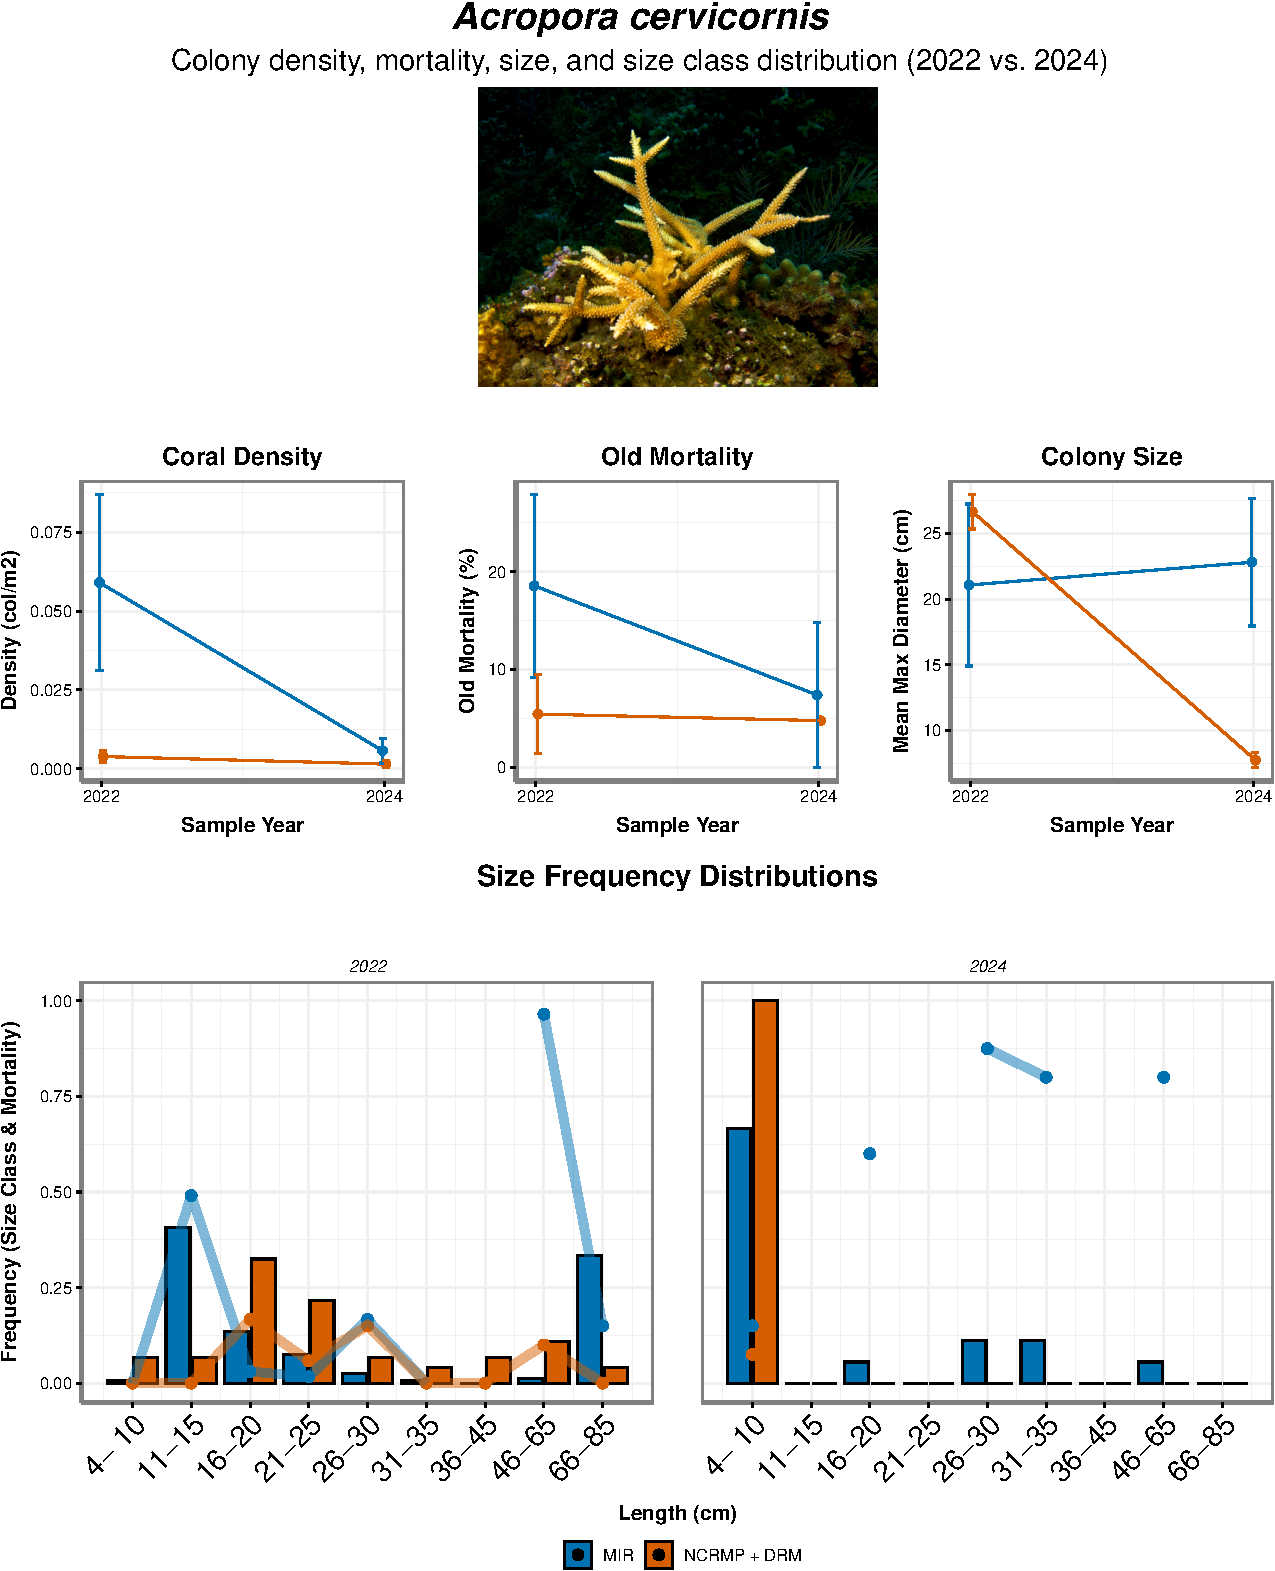
\includegraphics{MIR_quarto_files/figure-pdf/coral-tabyss-1.pdf}

}

\caption{Figures 3a-3i. Coral density, old mortality, colony size, and
size frequency distribution for focal M:IR species across sample years
(2022 and 2024) and survey types (MIR and NCRMP + DRM). Significant
difference in cover estimates in each of these areas was indicated by
(*).}

\end{figure}

\hypertarget{acropora-palmata}{%
\paragraph{\texorpdfstring{ Acropora palmata
}{ Acropora palmata }}\label{acropora-palmata}}

\begin{figure}

{\centering \includegraphics{MIR_quarto_files/figure-pdf/coral-tabyss-2.pdf}

}

\caption{Figures 3a-3i. Coral density, old mortality, colony size, and
size frequency distribution for focal M:IR species across sample years
(2022 and 2024) and survey types (MIR and NCRMP + DRM). Significant
difference in cover estimates in each of these areas was indicated by
(*).}

\end{figure}

\hypertarget{colpophyllia-natans}{%
\paragraph{\texorpdfstring{ Colpophyllia natans
}{ Colpophyllia natans }}\label{colpophyllia-natans}}

\begin{figure}

{\centering \includegraphics{MIR_quarto_files/figure-pdf/coral-tabyss-3.pdf}

}

\caption{Figures 3a-3i. Coral density, old mortality, colony size, and
size frequency distribution for focal M:IR species across sample years
(2022 and 2024) and survey types (MIR and NCRMP + DRM). Significant
difference in cover estimates in each of these areas was indicated by
(*).}

\end{figure}

\hypertarget{dichocoenia-stokesii}{%
\paragraph{\texorpdfstring{ Dichocoenia stokesii
}{ Dichocoenia stokesii }}\label{dichocoenia-stokesii}}

\begin{figure}

{\centering 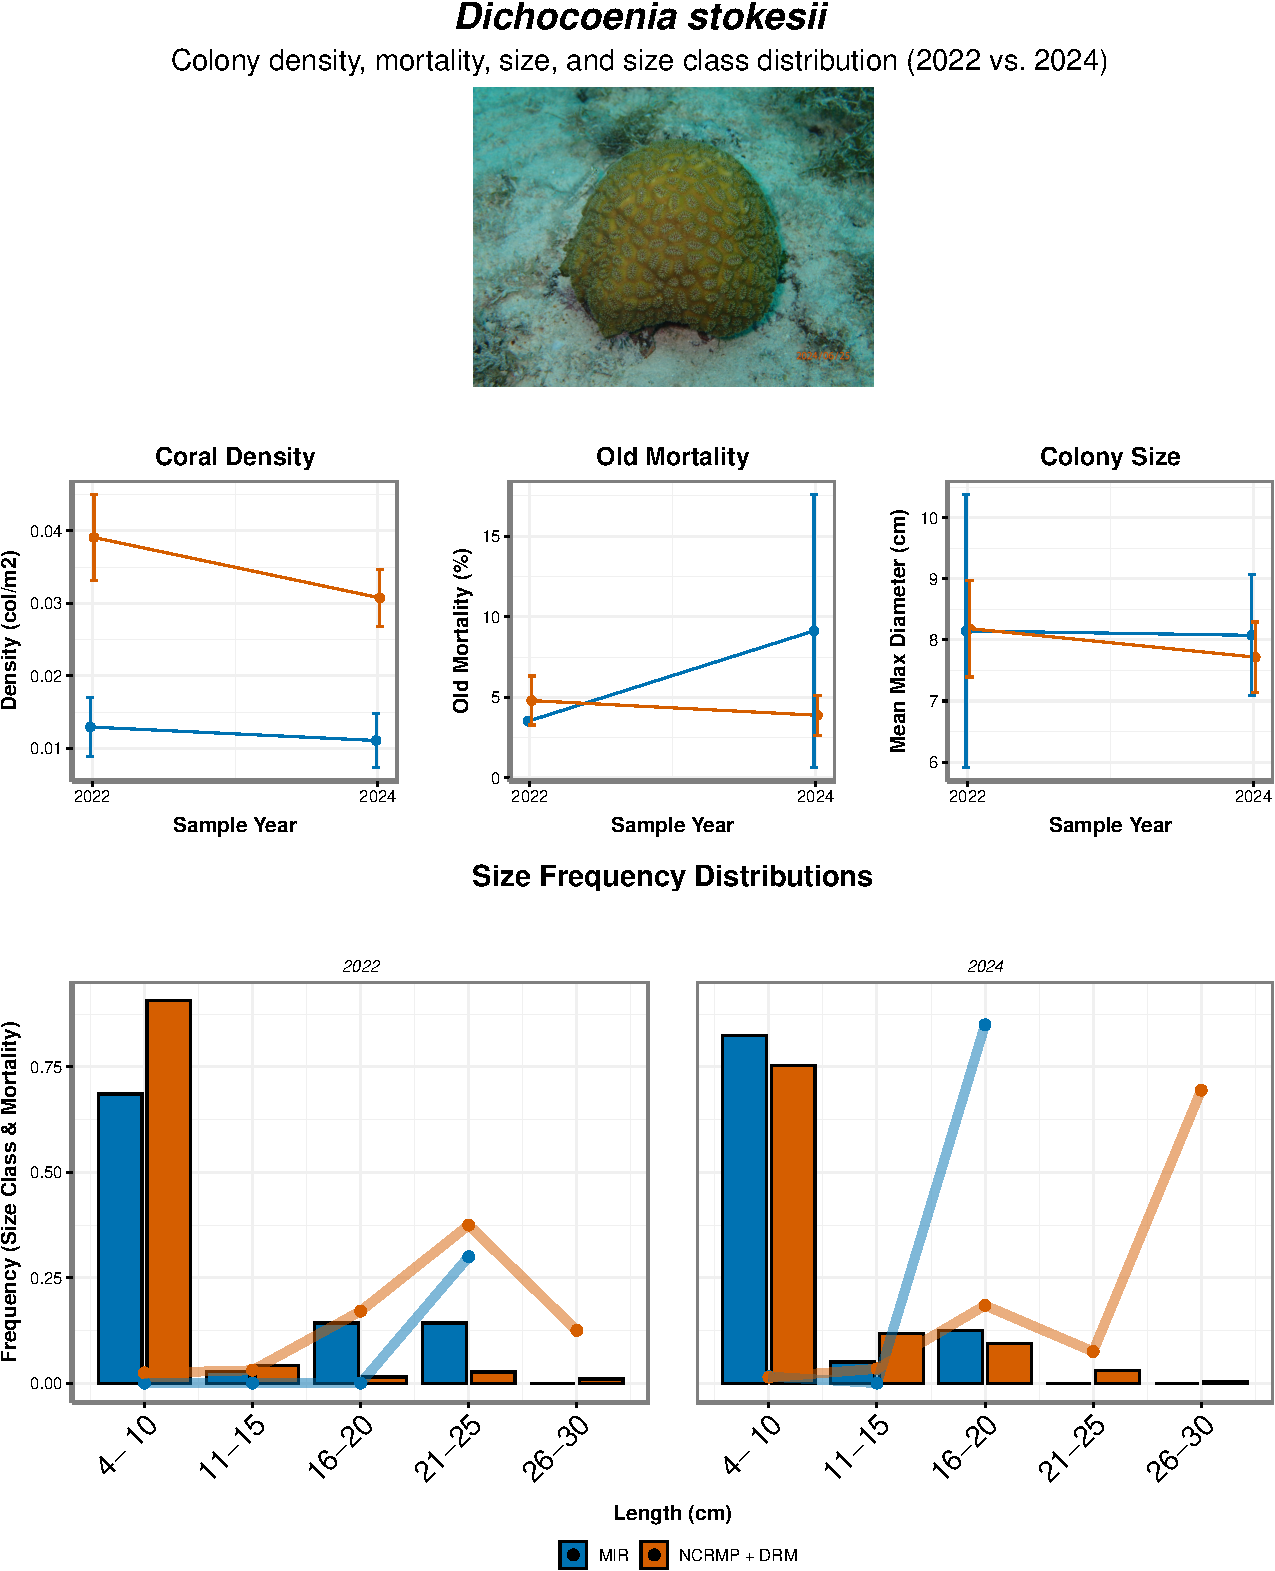
\includegraphics{MIR_quarto_files/figure-pdf/coral-tabyss-4.pdf}

}

\caption{Figures 3a-3i. Coral density, old mortality, colony size, and
size frequency distribution for focal M:IR species across sample years
(2022 and 2024) and survey types (MIR and NCRMP + DRM). Significant
difference in cover estimates in each of these areas was indicated by
(*).}

\end{figure}

\hypertarget{diploria-labyrinthiformis}{%
\paragraph{\texorpdfstring{ Diploria labyrinthiformis
}{ Diploria labyrinthiformis }}\label{diploria-labyrinthiformis}}

\begin{figure}

{\centering \includegraphics{MIR_quarto_files/figure-pdf/coral-tabyss-5.pdf}

}

\caption{Figures 3a-3i. Coral density, old mortality, colony size, and
size frequency distribution for focal M:IR species across sample years
(2022 and 2024) and survey types (MIR and NCRMP + DRM). Significant
difference in cover estimates in each of these areas was indicated by
(*).}

\end{figure}

\hypertarget{meandrina-meandrites}{%
\paragraph{\texorpdfstring{ Meandrina meandrites
}{ Meandrina meandrites }}\label{meandrina-meandrites}}

\begin{figure}

{\centering \includegraphics{MIR_quarto_files/figure-pdf/coral-tabyss-6.pdf}

}

\caption{Figures 3a-3i. Coral density, old mortality, colony size, and
size frequency distribution for focal M:IR species across sample years
(2022 and 2024) and survey types (MIR and NCRMP + DRM). Significant
difference in cover estimates in each of these areas was indicated by
(*).}

\end{figure}

\hypertarget{pseudodiploria-clivosa}{%
\paragraph{\texorpdfstring{ Pseudodiploria clivosa
}{ Pseudodiploria clivosa }}\label{pseudodiploria-clivosa}}

\begin{figure}

{\centering 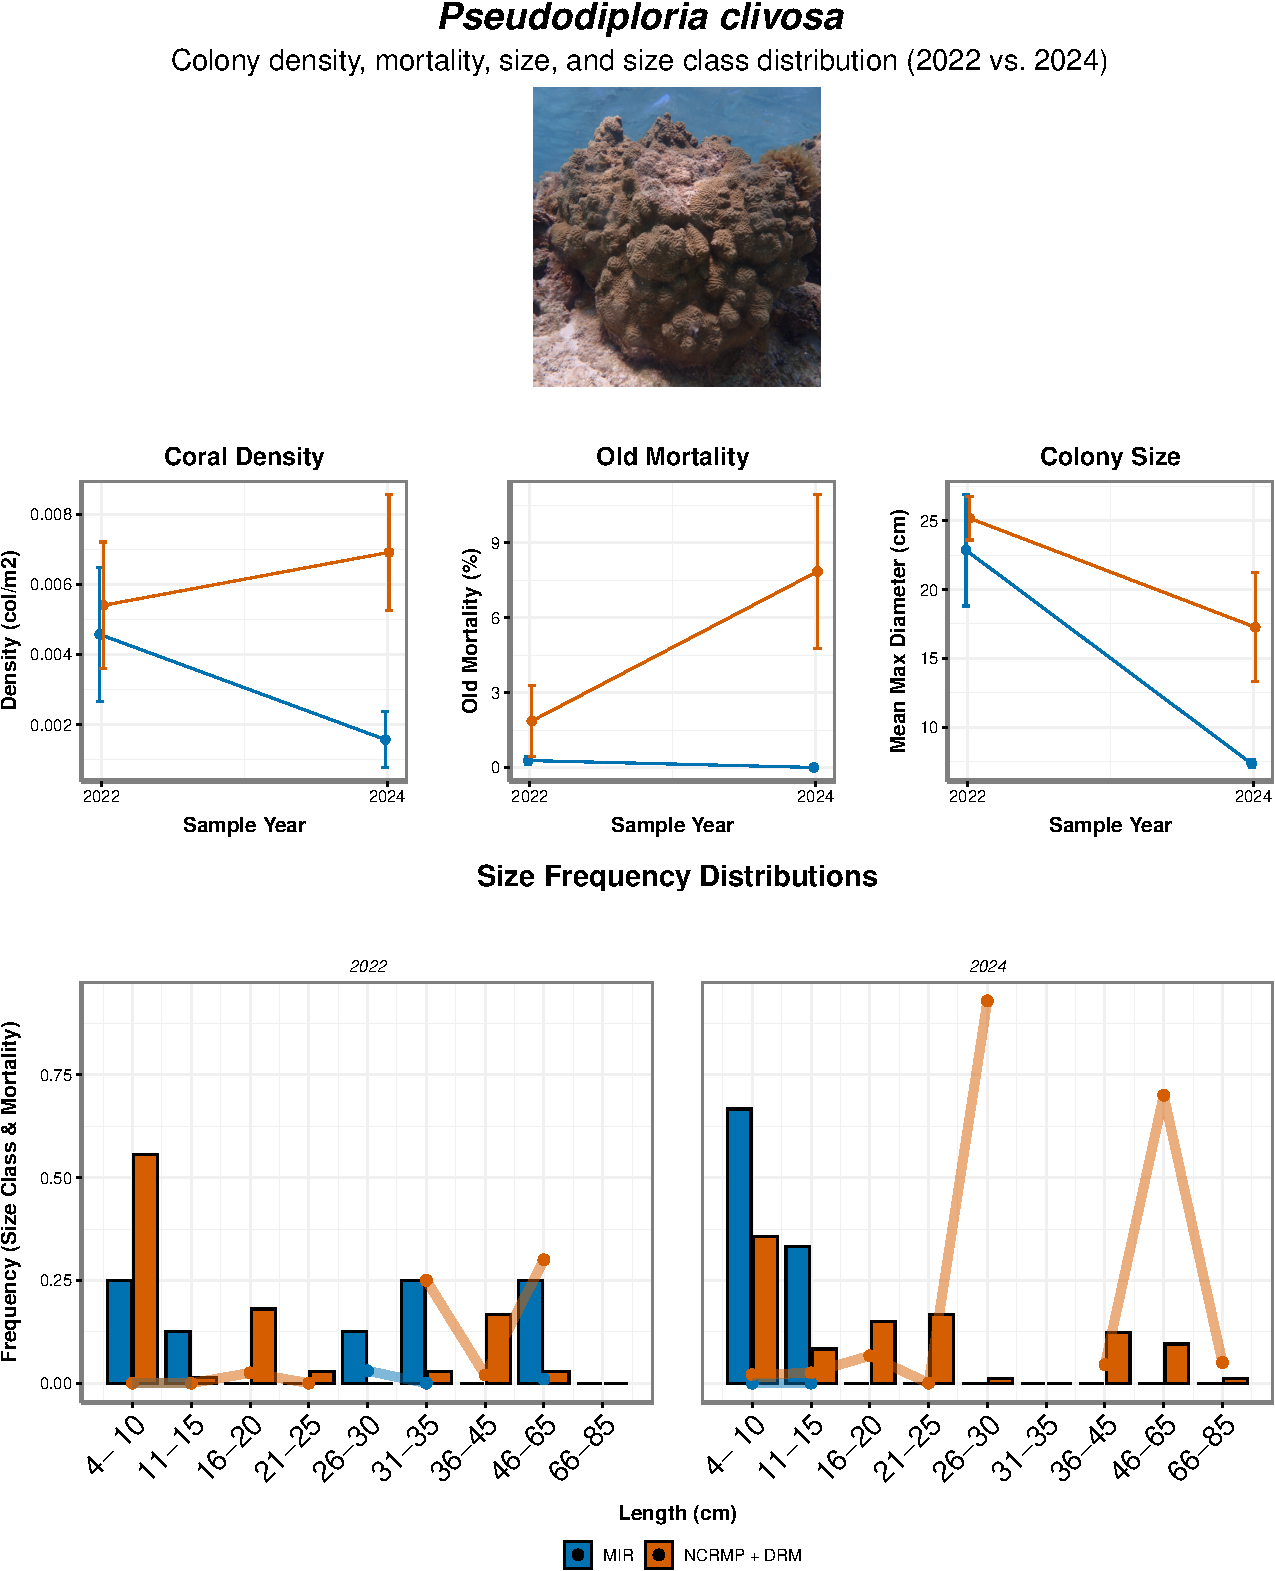
\includegraphics{MIR_quarto_files/figure-pdf/coral-tabyss-7.pdf}

}

\caption{Figures 3a-3i. Coral density, old mortality, colony size, and
size frequency distribution for focal M:IR species across sample years
(2022 and 2024) and survey types (MIR and NCRMP + DRM). Significant
difference in cover estimates in each of these areas was indicated by
(*).}

\end{figure}

\hypertarget{pseudodiploria-strigosa}{%
\paragraph{\texorpdfstring{ Pseudodiploria strigosa
}{ Pseudodiploria strigosa }}\label{pseudodiploria-strigosa}}

\begin{figure}

{\centering \includegraphics{MIR_quarto_files/figure-pdf/coral-tabyss-8.pdf}

}

\caption{Figures 3a-3i. Coral density, old mortality, colony size, and
size frequency distribution for focal M:IR species across sample years
(2022 and 2024) and survey types (MIR and NCRMP + DRM). Significant
difference in cover estimates in each of these areas was indicated by
(*).}

\end{figure}

\hypertarget{montastraea-cavernosa}{%
\paragraph{\texorpdfstring{ Montastraea cavernosa
}{ Montastraea cavernosa }}\label{montastraea-cavernosa}}

\begin{figure}

{\centering \includegraphics{MIR_quarto_files/figure-pdf/coral-tabyss-9.pdf}

}

\caption{Figures 3a-3i. Coral density, old mortality, colony size, and
size frequency distribution for focal M:IR species across sample years
(2022 and 2024) and survey types (MIR and NCRMP + DRM). Significant
difference in cover estimates in each of these areas was indicated by
(*).}

\end{figure}

\hypertarget{bleaching-estimates}{%
\subsection{Bleaching Estimates}\label{bleaching-estimates}}

\hypertarget{section}{%
\subsubsection{2022}\label{section}}

\begin{Shaded}
\begin{Highlighting}[]
\CommentTok{\# Set path to data files}
\NormalTok{data\_2022\_path }\OtherTok{\textless{}{-}} \StringTok{"data/FK2022\_NCRMP\_DRM\_MIR\_corsz\_ARallv2.csv"}



\NormalTok{MIR\_species }\OtherTok{\textless{}{-}} \FunctionTok{c}\NormalTok{(}\StringTok{"ACR PALM"}\NormalTok{, }\StringTok{"ACR CERV"}\NormalTok{, }\StringTok{"COL NATA"}\NormalTok{, }\StringTok{"DEN CYLI"}\NormalTok{, }\StringTok{"DIC STOK"}\NormalTok{, }\StringTok{"DIP LABY"}\NormalTok{, }\StringTok{"EUS FAST"}\NormalTok{, }\StringTok{"MEA MEAN"}\NormalTok{, }\StringTok{"PSE CLIV"}\NormalTok{, }\StringTok{"PSE STRI"}\NormalTok{, }\StringTok{"MON CAVE"}\NormalTok{)}

\CommentTok{\#Script works for the actual value but CI are not exact}
\CommentTok{\# tmp \textless{}{-} disease\_bleach\_prevalence\_ratio\_est(data\_2022\_path, 2022) \%\textgreater{}\%}
\CommentTok{\#   filter(PV\_TYPE == "Bleach\_All") \%\textgreater{}\%}
\CommentTok{\#   left\_join(., names)}


\NormalTok{names\_clean }\OtherTok{\textless{}{-}}\NormalTok{ names }\SpecialCharTok{\%\textgreater{}\%}
  \FunctionTok{select}\NormalTok{(SPECIES\_CD, SPECIES\_NAME) }\SpecialCharTok{\%\textgreater{}\%}
  \FunctionTok{distinct}\NormalTok{(SPECIES\_CD, }\AttributeTok{.keep\_all =} \ConstantTok{TRUE}\NormalTok{)}

\NormalTok{tmp\_ble\_2022 }\OtherTok{\textless{}{-}} \FunctionTok{read\_csv}\NormalTok{(}\StringTok{"data/fk2022\_NCRMP\_MIR\_sppPVbar\_Ball\_dom.csv"}\NormalTok{) }\SpecialCharTok{\%\textgreater{}\%}
  \FunctionTok{left\_join}\NormalTok{(., names\_clean, }\AttributeTok{by =} \StringTok{"SPECIES\_CD"}\NormalTok{)}

\NormalTok{top\_species }\OtherTok{\textless{}{-}}\NormalTok{ tmp\_ble\_2022 }\SpecialCharTok{\%\textgreater{}\%}
  \FunctionTok{group\_by}\NormalTok{(SPECIES\_CD) }\SpecialCharTok{\%\textgreater{}\%}
  \FunctionTok{summarise}\NormalTok{(}\AttributeTok{mean\_pv =} \FunctionTok{mean}\NormalTok{(PVbar, }\AttributeTok{na.rm =} \ConstantTok{TRUE}\NormalTok{)) }\SpecialCharTok{\%\textgreater{}\%}
  \FunctionTok{arrange}\NormalTok{(}\FunctionTok{desc}\NormalTok{(mean\_pv)) }\SpecialCharTok{\%\textgreater{}\%}
  \FunctionTok{slice\_head}\NormalTok{(}\AttributeTok{n =} \DecValTok{10}\NormalTok{) }\SpecialCharTok{\%\textgreater{}\%}  
  \FunctionTok{pull}\NormalTok{(SPECIES\_CD)}

\NormalTok{tmp\_filtered }\OtherTok{\textless{}{-}}\NormalTok{ tmp\_ble\_2022 }\SpecialCharTok{\%\textgreater{}\%}
  \FunctionTok{filter}\NormalTok{(SPECIES\_CD }\SpecialCharTok{\%in\%} \FunctionTok{union}\NormalTok{(top\_species, MIR\_species)) }

\DocumentationTok{\#\#Add a * for those MIR species}
\NormalTok{tmp\_filtered }\OtherTok{\textless{}{-}}\NormalTok{ tmp\_filtered }\SpecialCharTok{\%\textgreater{}\%} \FunctionTok{mutate}\NormalTok{(}
  \AttributeTok{SPECIES\_NAME =} \FunctionTok{case\_when}\NormalTok{(}
\NormalTok{    SPECIES\_CD }\SpecialCharTok{\%in\%}\NormalTok{ MIR\_species }\SpecialCharTok{\textasciitilde{}} \FunctionTok{paste0}\NormalTok{(}\StringTok{"*"}\NormalTok{, SPECIES\_NAME),}
    \ConstantTok{TRUE} \SpecialCharTok{\textasciitilde{}} \FunctionTok{as.character}\NormalTok{(SPECIES\_NAME)))}

\CommentTok{\#Factor re{-}order for aesthetics  }
\NormalTok{tmp\_filtered }\OtherTok{\textless{}{-}}\NormalTok{ tmp\_filtered }\SpecialCharTok{\%\textgreater{}\%}
  \FunctionTok{mutate}\NormalTok{(}\AttributeTok{SPECIES\_NAME =} 
           \FunctionTok{fct\_reorder}\NormalTok{(SPECIES\_NAME, }\FunctionTok{if\_else}\NormalTok{(}\FunctionTok{is.na}\NormalTok{(PVbar), }\DecValTok{0}\NormalTok{, PVbar), }\AttributeTok{.desc =} \ConstantTok{FALSE}\NormalTok{))}

\NormalTok{plt\_bleach }\OtherTok{\textless{}{-}}\NormalTok{ tmp\_filtered }\SpecialCharTok{\%\textgreater{}\%}
  \FunctionTok{filter}\NormalTok{(SPECIES\_NAME }\SpecialCharTok{!=} \StringTok{"NA"}\NormalTok{) }\SpecialCharTok{\%\textgreater{}\%}
  \FunctionTok{ggplot}\NormalTok{(}\FunctionTok{aes}\NormalTok{(}\AttributeTok{x =}\NormalTok{ PVbar, }\AttributeTok{y =}\NormalTok{ SPECIES\_NAME, }\AttributeTok{fill =}\NormalTok{ analysis\_group )) }\SpecialCharTok{+}
  \FunctionTok{geom\_col}\NormalTok{(}\AttributeTok{position =} \FunctionTok{position\_dodge}\NormalTok{(}\AttributeTok{width =} \FloatTok{0.8}\NormalTok{), }\AttributeTok{width =} \FloatTok{0.8}\NormalTok{) }\SpecialCharTok{+}
  \FunctionTok{scale\_fill\_manual}\NormalTok{(}\AttributeTok{values =} \FunctionTok{c}\NormalTok{(}\StringTok{"\#0072B2"}\NormalTok{, }\StringTok{"\#D55E00"}\NormalTok{), }\AttributeTok{labels =} \FunctionTok{c}\NormalTok{(}\StringTok{"MIR"}\NormalTok{, }\StringTok{"NCRMP + DRM"}\NormalTok{)) }\SpecialCharTok{+}
  \FunctionTok{geom\_errorbar}\NormalTok{(}\FunctionTok{aes}\NormalTok{(}\AttributeTok{xmin =}\NormalTok{ PV\_LCI, }\AttributeTok{xmax =}\NormalTok{ PV\_UCI),}
                \AttributeTok{position =} \FunctionTok{position\_dodge}\NormalTok{(}\AttributeTok{width =} \FloatTok{0.8}\NormalTok{), }\AttributeTok{width =} \FloatTok{0.1}\NormalTok{) }\SpecialCharTok{+}
  \FunctionTok{facet\_wrap}\NormalTok{(}\SpecialCharTok{\textasciitilde{}}\NormalTok{analysis\_group) }\SpecialCharTok{+}
    \FunctionTok{labs}\NormalTok{(}\AttributeTok{x =} \StringTok{"Proportion of Colonies Bleached"}\NormalTok{, }\AttributeTok{y =} \StringTok{"Coral Species"}\NormalTok{, }\AttributeTok{fill =} \StringTok{""}\NormalTok{) }\SpecialCharTok{+}
    \FunctionTok{scale\_x\_continuous}\NormalTok{(}\AttributeTok{expand =} \FunctionTok{expansion}\NormalTok{(}\AttributeTok{mult =} \FunctionTok{c}\NormalTok{(}\DecValTok{0}\NormalTok{, }\FloatTok{0.1}\NormalTok{))) }\SpecialCharTok{+}
        \FunctionTok{theme\_Publication}\NormalTok{(}\AttributeTok{base\_size =} \DecValTok{10}\NormalTok{) }\SpecialCharTok{+}
    \FunctionTok{coord\_cartesian}\NormalTok{(}\AttributeTok{clip =} \StringTok{"off"}\NormalTok{) }\SpecialCharTok{+}
        \FunctionTok{scale\_y\_discrete}\NormalTok{(}\AttributeTok{labels =} \ControlFlowTok{function}\NormalTok{(x) }\FunctionTok{parse}\NormalTok{(}\AttributeTok{text =} \FunctionTok{paste0}\NormalTok{(}\StringTok{"italic(\textquotesingle{}"}\NormalTok{, x, }\StringTok{"\textquotesingle{})"}\NormalTok{))) }\SpecialCharTok{+}
    \FunctionTok{theme}\NormalTok{(}
          \AttributeTok{strip.text =} \FunctionTok{element\_text}\NormalTok{(}\AttributeTok{size =} \DecValTok{14}\NormalTok{, }\AttributeTok{face =} \StringTok{"bold"}\NormalTok{),}
          \AttributeTok{axis.text.y =} \FunctionTok{element\_text}\NormalTok{(}\AttributeTok{size =} \DecValTok{11}\NormalTok{),}
          \AttributeTok{axis.title =} \FunctionTok{element\_text}\NormalTok{(}\AttributeTok{size =} \DecValTok{13}\NormalTok{),}
          \AttributeTok{legend.position =} \StringTok{"bottom"}\NormalTok{,}
          \AttributeTok{legend.text =} \FunctionTok{element\_text}\NormalTok{(}\AttributeTok{size =} \DecValTok{10}\NormalTok{),}
          \AttributeTok{panel.spacing =} \FunctionTok{unit}\NormalTok{(}\DecValTok{1}\NormalTok{, }\StringTok{"lines"}\NormalTok{)}
\NormalTok{        ) }\CommentTok{\#+}
 \CommentTok{\# ggtitle("2022 Estimates")}


\FunctionTok{print}\NormalTok{(plt\_bleach)}
\end{Highlighting}
\end{Shaded}

\begin{figure}[H]

{\centering \includegraphics{MIR_quarto_files/figure-pdf/bleach 2022-1.pdf}

}

\caption{Figure 4. Estimated Observed Bleaching Frequency in 2022 using
Ratio Estimaters.}

\end{figure}

\hypertarget{section-1}{%
\subsubsection{2024}\label{section-1}}

\begin{Shaded}
\begin{Highlighting}[]
\CommentTok{\# Set path to data files}
\NormalTok{data\_2022\_path }\OtherTok{\textless{}{-}} \StringTok{"data/FK2022\_NCRMP\_DRM\_MIR\_corsz\_ARallv2.csv"}


\NormalTok{MIR\_species }\OtherTok{\textless{}{-}} \FunctionTok{c}\NormalTok{(}\StringTok{"ACR PALM"}\NormalTok{, }\StringTok{"ACR CERV"}\NormalTok{, }\StringTok{"COL NATA"}\NormalTok{, }\StringTok{"DEN CYLI"}\NormalTok{, }\StringTok{"DIC STOK"}\NormalTok{, }\StringTok{"DIP LABY"}\NormalTok{, }\StringTok{"EUS FAST"}\NormalTok{, }\StringTok{"MEA MEAN"}\NormalTok{, }\StringTok{"PSE CLIV"}\NormalTok{, }\StringTok{"PSE STRI"}\NormalTok{, }\StringTok{"MON CAVE"}\NormalTok{)}

\CommentTok{\#same as section above}
\CommentTok{\# tmp \textless{}{-} disease\_bleach\_prevalence\_ratio\_est(data\_2022\_path, 2022) \%\textgreater{}\%}
\CommentTok{\#   filter(PV\_TYPE == "Bleach\_All") \%\textgreater{}\%}
\CommentTok{\#   left\_join(., names)}

\NormalTok{names\_clean }\OtherTok{\textless{}{-}}\NormalTok{ names }\SpecialCharTok{\%\textgreater{}\%}
  \FunctionTok{select}\NormalTok{(SPECIES\_CD, SPECIES\_NAME) }\SpecialCharTok{\%\textgreater{}\%}
  \FunctionTok{distinct}\NormalTok{(SPECIES\_CD, }\AttributeTok{.keep\_all =} \ConstantTok{TRUE}\NormalTok{)}

\NormalTok{tmp }\OtherTok{\textless{}{-}} \FunctionTok{read\_csv}\NormalTok{(}\StringTok{"data/fk2024\_NCRMP\_MIR\_sppPVbar\_Ball\_dom.csv"}\NormalTok{) }\SpecialCharTok{\%\textgreater{}\%}
    \FunctionTok{left\_join}\NormalTok{(names\_clean, }\AttributeTok{by =} \StringTok{"SPECIES\_CD"}\NormalTok{)}

\NormalTok{top\_species }\OtherTok{\textless{}{-}}\NormalTok{ tmp }\SpecialCharTok{\%\textgreater{}\%}
  \FunctionTok{group\_by}\NormalTok{(SPECIES\_CD) }\SpecialCharTok{\%\textgreater{}\%}
  \FunctionTok{summarise}\NormalTok{(}\AttributeTok{mean\_pv =} \FunctionTok{mean}\NormalTok{(PVbar, }\AttributeTok{na.rm =} \ConstantTok{TRUE}\NormalTok{)) }\SpecialCharTok{\%\textgreater{}\%}
  \FunctionTok{arrange}\NormalTok{(}\FunctionTok{desc}\NormalTok{(mean\_pv)) }\SpecialCharTok{\%\textgreater{}\%}
  \FunctionTok{slice\_head}\NormalTok{(}\AttributeTok{n =} \DecValTok{10}\NormalTok{) }\SpecialCharTok{\%\textgreater{}\%}  
  \FunctionTok{pull}\NormalTok{(SPECIES\_CD)}

\NormalTok{tmp\_filtered }\OtherTok{\textless{}{-}}\NormalTok{ tmp }\SpecialCharTok{\%\textgreater{}\%}
  \FunctionTok{filter}\NormalTok{(SPECIES\_CD }\SpecialCharTok{\%in\%} \FunctionTok{union}\NormalTok{(top\_species, MIR\_species)) }
  
\DocumentationTok{\#\#Add a * for those MIR species}
\NormalTok{tmp\_filtered }\OtherTok{\textless{}{-}}\NormalTok{ tmp\_filtered }\SpecialCharTok{\%\textgreater{}\%} \FunctionTok{mutate}\NormalTok{(}
  \AttributeTok{SPECIES\_NAME =} \FunctionTok{case\_when}\NormalTok{(}
\NormalTok{    SPECIES\_CD }\SpecialCharTok{\%in\%}\NormalTok{ MIR\_species }\SpecialCharTok{\textasciitilde{}} \FunctionTok{paste0}\NormalTok{(}\StringTok{"*"}\NormalTok{, SPECIES\_NAME),}
    \ConstantTok{TRUE} \SpecialCharTok{\textasciitilde{}} \FunctionTok{as.character}\NormalTok{(SPECIES\_NAME)))}

\CommentTok{\#Factor re{-}order for aesthetics  }
\NormalTok{tmp\_filtered }\OtherTok{\textless{}{-}}\NormalTok{ tmp\_filtered }\SpecialCharTok{\%\textgreater{}\%}
  \FunctionTok{mutate}\NormalTok{(}\AttributeTok{SPECIES\_NAME =} 
           \FunctionTok{fct\_reorder}\NormalTok{(SPECIES\_NAME, }\FunctionTok{if\_else}\NormalTok{(}\FunctionTok{is.na}\NormalTok{(PVbar), }\DecValTok{0}\NormalTok{, PVbar), }\AttributeTok{.desc =} \ConstantTok{FALSE}\NormalTok{))}

\NormalTok{plt\_bleach }\OtherTok{\textless{}{-}}\NormalTok{ tmp\_filtered }\SpecialCharTok{\%\textgreater{}\%}
  \FunctionTok{filter}\NormalTok{(SPECIES\_NAME }\SpecialCharTok{!=} \StringTok{"NA"}\NormalTok{) }\SpecialCharTok{\%\textgreater{}\%}
  \FunctionTok{ggplot}\NormalTok{(}\FunctionTok{aes}\NormalTok{(}\AttributeTok{x =}\NormalTok{ PVbar, }\AttributeTok{y =}\NormalTok{ SPECIES\_NAME, }\AttributeTok{fill =}\NormalTok{ analysis\_group)) }\SpecialCharTok{+}
  \FunctionTok{geom\_col}\NormalTok{(}\AttributeTok{position =} \FunctionTok{position\_dodge}\NormalTok{(}\AttributeTok{width =} \FloatTok{0.8}\NormalTok{), }\AttributeTok{width =} \FloatTok{0.8}\NormalTok{) }\SpecialCharTok{+}
  \FunctionTok{geom\_errorbar}\NormalTok{(}\FunctionTok{aes}\NormalTok{(}\AttributeTok{xmin =}\NormalTok{ PV\_LCI, }\AttributeTok{xmax =}\NormalTok{ PV\_UCI),}
                \AttributeTok{position =} \FunctionTok{position\_dodge}\NormalTok{(}\AttributeTok{width =} \FloatTok{0.8}\NormalTok{), }\AttributeTok{width =} \FloatTok{0.1}\NormalTok{) }\SpecialCharTok{+}
  \FunctionTok{facet\_wrap}\NormalTok{(}\SpecialCharTok{\textasciitilde{}}\NormalTok{analysis\_group) }\SpecialCharTok{+}
    \FunctionTok{labs}\NormalTok{(}\AttributeTok{x =} \StringTok{"Proportion of Colonies Bleached"}\NormalTok{, }\AttributeTok{y =} \StringTok{"Coral Species"}\NormalTok{, }\AttributeTok{fill =} \StringTok{""}\NormalTok{) }\SpecialCharTok{+}
    \FunctionTok{scale\_x\_continuous}\NormalTok{(}\AttributeTok{expand =} \FunctionTok{expansion}\NormalTok{(}\AttributeTok{mult =} \FunctionTok{c}\NormalTok{(}\DecValTok{0}\NormalTok{, }\FloatTok{0.1}\NormalTok{))) }\SpecialCharTok{+}
        \FunctionTok{theme\_Publication}\NormalTok{(}\AttributeTok{base\_size =} \DecValTok{10}\NormalTok{) }\SpecialCharTok{+}
    \FunctionTok{coord\_cartesian}\NormalTok{(}\AttributeTok{clip =} \StringTok{"off"}\NormalTok{) }\SpecialCharTok{+}
        \FunctionTok{scale\_y\_discrete}\NormalTok{(}\AttributeTok{labels =} \ControlFlowTok{function}\NormalTok{(x) }\FunctionTok{parse}\NormalTok{(}\AttributeTok{text =} \FunctionTok{paste0}\NormalTok{(}\StringTok{"italic(\textquotesingle{}"}\NormalTok{, x, }\StringTok{"\textquotesingle{})"}\NormalTok{))) }\SpecialCharTok{+}
   \FunctionTok{scale\_fill\_manual}\NormalTok{(}\AttributeTok{values =} \FunctionTok{c}\NormalTok{(}\StringTok{"\#0072B2"}\NormalTok{, }\StringTok{"\#D55E00"}\NormalTok{), }\AttributeTok{labels =} \FunctionTok{c}\NormalTok{(}\StringTok{"MIR"}\NormalTok{, }\StringTok{"NCRMP + DRM"}\NormalTok{)) }\SpecialCharTok{+}
    \FunctionTok{theme}\NormalTok{(}
          \AttributeTok{strip.text =} \FunctionTok{element\_text}\NormalTok{(}\AttributeTok{size =} \DecValTok{14}\NormalTok{, }\AttributeTok{face =} \StringTok{"bold"}\NormalTok{),}
          \AttributeTok{axis.text.y =} \FunctionTok{element\_text}\NormalTok{(}\AttributeTok{size =} \DecValTok{11}\NormalTok{),}
          \AttributeTok{axis.title =} \FunctionTok{element\_text}\NormalTok{(}\AttributeTok{size =} \DecValTok{13}\NormalTok{),}
          \AttributeTok{legend.position =} \StringTok{"bottom"}\NormalTok{,}
          \AttributeTok{legend.text =} \FunctionTok{element\_text}\NormalTok{(}\AttributeTok{size =} \DecValTok{10}\NormalTok{),}
          \AttributeTok{panel.spacing =} \FunctionTok{unit}\NormalTok{(}\DecValTok{1}\NormalTok{, }\StringTok{"lines"}\NormalTok{)}
\NormalTok{        ) }\CommentTok{\#+}
  \CommentTok{\#ggtitle("2024 Estimates")}


\FunctionTok{print}\NormalTok{(plt\_bleach)}
\end{Highlighting}
\end{Shaded}

\begin{figure}[H]

{\centering \includegraphics{MIR_quarto_files/figure-pdf/bleach 2024-1.pdf}

}

\caption{Figure 5. Estimated Observed Bleaching Frequency in 2024 using
Ratio Estimaters}

\end{figure}

\hypertarget{disease-estimates}{%
\subsection{Disease Estimates}\label{disease-estimates}}

\hypertarget{section-2}{%
\subsubsection{2022}\label{section-2}}

\begin{Shaded}
\begin{Highlighting}[]
\CommentTok{\# Set path to data files}
\NormalTok{data\_2022\_path }\OtherTok{\textless{}{-}} \StringTok{"data/FK2022\_NCRMP\_DRM\_MIR\_corsz\_ARallv2.csv"}


\NormalTok{MIR\_species }\OtherTok{\textless{}{-}} \FunctionTok{c}\NormalTok{(}\StringTok{"ACR PALM"}\NormalTok{, }\StringTok{"ACR CERV"}\NormalTok{, }\StringTok{"COL NATA"}\NormalTok{, }\StringTok{"DEN CYLI"}\NormalTok{, }\StringTok{"DIC STOK"}\NormalTok{, }\StringTok{"DIP LABY"}\NormalTok{, }\StringTok{"EUS FAST"}\NormalTok{, }\StringTok{"MEA MEAN"}\NormalTok{, }\StringTok{"PSE CLIV"}\NormalTok{, }\StringTok{"PSE STRI"}\NormalTok{, }\StringTok{"MON CAVE"}\NormalTok{)}

\CommentTok{\# tmp \textless{}{-} disease\_bleach\_prevalence\_ratio\_est(data\_2022\_path, 2022) \%\textgreater{}\%}
\CommentTok{\#   filter(PV\_TYPE == "Bleach\_All") \%\textgreater{}\%}
\CommentTok{\#   left\_join(., names)}

\NormalTok{names\_clean }\OtherTok{\textless{}{-}}\NormalTok{ names }\SpecialCharTok{\%\textgreater{}\%}
  \FunctionTok{select}\NormalTok{(SPECIES\_CD, SPECIES\_NAME) }\SpecialCharTok{\%\textgreater{}\%}
  \FunctionTok{distinct}\NormalTok{(SPECIES\_CD, }\AttributeTok{.keep\_all =} \ConstantTok{TRUE}\NormalTok{)}

\NormalTok{tmp\_dis\_2022 }\OtherTok{\textless{}{-}} \FunctionTok{read\_csv}\NormalTok{(}\StringTok{"data/fk2022\_NCRMP\_MIR\_sppPVbar\_Dall\_dom.csv"}\NormalTok{) }\SpecialCharTok{\%\textgreater{}\%}
    \FunctionTok{left\_join}\NormalTok{(names\_clean, }\AttributeTok{by =} \StringTok{"SPECIES\_CD"}\NormalTok{)}

\NormalTok{top\_species }\OtherTok{\textless{}{-}}\NormalTok{ tmp\_dis\_2022 }\SpecialCharTok{\%\textgreater{}\%}
  \FunctionTok{group\_by}\NormalTok{(SPECIES\_CD) }\SpecialCharTok{\%\textgreater{}\%}
  \FunctionTok{summarise}\NormalTok{(}\AttributeTok{mean\_pv =} \FunctionTok{mean}\NormalTok{(PVbar, }\AttributeTok{na.rm =} \ConstantTok{TRUE}\NormalTok{)) }\SpecialCharTok{\%\textgreater{}\%}
  \FunctionTok{arrange}\NormalTok{(}\FunctionTok{desc}\NormalTok{(mean\_pv)) }\SpecialCharTok{\%\textgreater{}\%}
  \FunctionTok{slice\_head}\NormalTok{(}\AttributeTok{n =} \DecValTok{10}\NormalTok{) }\SpecialCharTok{\%\textgreater{}\%}  
  \FunctionTok{pull}\NormalTok{(SPECIES\_CD)}

\NormalTok{tmp\_filtered }\OtherTok{\textless{}{-}}\NormalTok{ tmp\_dis\_2022 }\SpecialCharTok{\%\textgreater{}\%}
  \FunctionTok{filter}\NormalTok{(SPECIES\_CD }\SpecialCharTok{\%in\%} \FunctionTok{union}\NormalTok{(top\_species, MIR\_species)) }
  
\DocumentationTok{\#\#Add a * for those MIR species}
\NormalTok{tmp\_filtered }\OtherTok{\textless{}{-}}\NormalTok{ tmp\_filtered }\SpecialCharTok{\%\textgreater{}\%} \FunctionTok{mutate}\NormalTok{(}
  \AttributeTok{SPECIES\_NAME =} \FunctionTok{case\_when}\NormalTok{(}
\NormalTok{    SPECIES\_CD }\SpecialCharTok{\%in\%}\NormalTok{ MIR\_species }\SpecialCharTok{\textasciitilde{}} \FunctionTok{paste0}\NormalTok{( }\StringTok{"*"}\NormalTok{, SPECIES\_NAME),}
    \ConstantTok{TRUE} \SpecialCharTok{\textasciitilde{}} \FunctionTok{as.character}\NormalTok{(SPECIES\_NAME)))}

\CommentTok{\#Factor re{-}order for aesthetics  }
\NormalTok{tmp\_filtered }\OtherTok{\textless{}{-}}\NormalTok{ tmp\_filtered }\SpecialCharTok{\%\textgreater{}\%}
  \FunctionTok{mutate}\NormalTok{(}\AttributeTok{SPECIES\_NAME =} 
           \FunctionTok{fct\_reorder}\NormalTok{(SPECIES\_NAME, }\FunctionTok{if\_else}\NormalTok{(}\FunctionTok{is.na}\NormalTok{(PVbar), }\DecValTok{0}\NormalTok{, PVbar), }\AttributeTok{.desc =} \ConstantTok{FALSE}\NormalTok{))}

\NormalTok{plt\_disease }\OtherTok{\textless{}{-}}\NormalTok{ tmp\_filtered }\SpecialCharTok{\%\textgreater{}\%}
  \FunctionTok{filter}\NormalTok{(SPECIES\_NAME }\SpecialCharTok{!=} \StringTok{"NA"}\NormalTok{) }\SpecialCharTok{\%\textgreater{}\%}
  \FunctionTok{ggplot}\NormalTok{(}\FunctionTok{aes}\NormalTok{(}\AttributeTok{x =}\NormalTok{ PVbar, }\AttributeTok{y =}\NormalTok{ SPECIES\_NAME, }\AttributeTok{fill =}\NormalTok{ analysis\_group)) }\SpecialCharTok{+}
  \FunctionTok{geom\_col}\NormalTok{(}\AttributeTok{position =} \FunctionTok{position\_dodge}\NormalTok{(}\AttributeTok{width =} \FloatTok{0.8}\NormalTok{), }\AttributeTok{width =} \FloatTok{0.8}\NormalTok{) }\SpecialCharTok{+}
  \FunctionTok{geom\_errorbar}\NormalTok{(}
    \FunctionTok{aes}\NormalTok{(}\AttributeTok{xmin =} \FunctionTok{pmax}\NormalTok{(}\DecValTok{0}\NormalTok{, PV\_LCI), }\AttributeTok{xmax =}\NormalTok{ PV\_UCI),}
    \AttributeTok{width =} \FloatTok{0.15}
\NormalTok{  ) }\SpecialCharTok{+}
  \FunctionTok{facet\_wrap}\NormalTok{(}\SpecialCharTok{\textasciitilde{}}\NormalTok{analysis\_group) }\SpecialCharTok{+}
    \FunctionTok{labs}\NormalTok{(}\AttributeTok{x =} \StringTok{"Proportion of Colonies Bleached"}\NormalTok{, }\AttributeTok{y =} \StringTok{"Coral Species"}\NormalTok{, }\AttributeTok{fill =} \StringTok{""}\NormalTok{) }\SpecialCharTok{+}
    \FunctionTok{scale\_x\_continuous}\NormalTok{(}\AttributeTok{expand =} \FunctionTok{expansion}\NormalTok{(}\AttributeTok{mult =} \FunctionTok{c}\NormalTok{(}\DecValTok{0}\NormalTok{, }\FloatTok{0.1}\NormalTok{))) }\SpecialCharTok{+}
        \FunctionTok{theme\_Publication}\NormalTok{(}\AttributeTok{base\_size =} \DecValTok{10}\NormalTok{) }\SpecialCharTok{+}
    \FunctionTok{coord\_cartesian}\NormalTok{(}\AttributeTok{clip =} \StringTok{"off"}\NormalTok{) }\SpecialCharTok{+}
        \FunctionTok{scale\_y\_discrete}\NormalTok{(}\AttributeTok{labels =} \ControlFlowTok{function}\NormalTok{(x) }\FunctionTok{parse}\NormalTok{(}\AttributeTok{text =} \FunctionTok{paste0}\NormalTok{(}\StringTok{"italic(\textquotesingle{}"}\NormalTok{, x, }\StringTok{"\textquotesingle{})"}\NormalTok{))) }\SpecialCharTok{+}
   \FunctionTok{scale\_fill\_manual}\NormalTok{(}\AttributeTok{values =} \FunctionTok{c}\NormalTok{(}\StringTok{"\#0072B2"}\NormalTok{, }\StringTok{"\#D55E00"}\NormalTok{), }\AttributeTok{labels =} \FunctionTok{c}\NormalTok{(}\StringTok{"MIR"}\NormalTok{, }\StringTok{"NCRMP + DRM"}\NormalTok{)) }\SpecialCharTok{+}
    \FunctionTok{theme}\NormalTok{(}
          \AttributeTok{strip.text =} \FunctionTok{element\_text}\NormalTok{(}\AttributeTok{size =} \DecValTok{14}\NormalTok{, }\AttributeTok{face =} \StringTok{"bold"}\NormalTok{),}
          \AttributeTok{axis.text.y =} \FunctionTok{element\_text}\NormalTok{(}\AttributeTok{size =} \DecValTok{11}\NormalTok{),}
          \AttributeTok{axis.title =} \FunctionTok{element\_text}\NormalTok{(}\AttributeTok{size =} \DecValTok{13}\NormalTok{),}
          \AttributeTok{legend.position =} \StringTok{"bottom"}\NormalTok{,}
          \AttributeTok{legend.text =} \FunctionTok{element\_text}\NormalTok{(}\AttributeTok{size =} \DecValTok{10}\NormalTok{),}
          \AttributeTok{panel.spacing =} \FunctionTok{unit}\NormalTok{(}\DecValTok{1}\NormalTok{, }\StringTok{"lines"}\NormalTok{)}
\NormalTok{        ) }\CommentTok{\#+}
  \CommentTok{\#ggtitle("2022 Estimates")}


\FunctionTok{print}\NormalTok{(plt\_disease)}
\end{Highlighting}
\end{Shaded}

\begin{figure}[H]

{\centering \includegraphics{MIR_quarto_files/figure-pdf/disease 2024-1.pdf}

}

\caption{Figure 6 . Estimated Observed Disease Frequency in 2022 using
Ratio Estimaters.}

\end{figure}

\hypertarget{section-3}{%
\subsubsection{2024}\label{section-3}}

\begin{Shaded}
\begin{Highlighting}[]
\CommentTok{\# Set path to data files}
\NormalTok{data\_2024\_path }\OtherTok{\textless{}{-}} \StringTok{"data/FK2022\_NCRMP\_DRM\_MIR\_corsz\_ARallv2.csv"}


\NormalTok{MIR\_species }\OtherTok{\textless{}{-}} \FunctionTok{c}\NormalTok{(}\StringTok{"ACR PALM"}\NormalTok{, }\StringTok{"ACR CERV"}\NormalTok{, }\StringTok{"COL NATA"}\NormalTok{, }\StringTok{"DEN CYLI"}\NormalTok{, }\StringTok{"DIC STOK"}\NormalTok{, }\StringTok{"DIP LABY"}\NormalTok{, }\StringTok{"EUS FAST"}\NormalTok{, }\StringTok{"MEA MEAN"}\NormalTok{, }\StringTok{"PSE CLIV"}\NormalTok{, }\StringTok{"PSE STRI"}\NormalTok{, }\StringTok{"MON CAVE"}\NormalTok{)}

\CommentTok{\# tmp \textless{}{-} disease\_bleach\_prevalence\_ratio\_est(data\_2022\_path, 2022) \%\textgreater{}\%}
\CommentTok{\#   filter(PV\_TYPE == "Bleach\_All") \%\textgreater{}\%}
\CommentTok{\#   left\_join(., names)}

\NormalTok{names\_clean }\OtherTok{\textless{}{-}}\NormalTok{ names }\SpecialCharTok{\%\textgreater{}\%}
  \FunctionTok{select}\NormalTok{(SPECIES\_CD, SPECIES\_NAME) }\SpecialCharTok{\%\textgreater{}\%}
  \FunctionTok{distinct}\NormalTok{(SPECIES\_CD, }\AttributeTok{.keep\_all =} \ConstantTok{TRUE}\NormalTok{)}

\NormalTok{tmp\_dis\_2024 }\OtherTok{\textless{}{-}} \FunctionTok{read\_csv}\NormalTok{(}\StringTok{"data/fk2024\_NCRMP\_MIR\_sppPVbar\_Dall\_dom.csv"}\NormalTok{) }\SpecialCharTok{\%\textgreater{}\%}
    \FunctionTok{left\_join}\NormalTok{(names\_clean, }\AttributeTok{by =} \StringTok{"SPECIES\_CD"}\NormalTok{)}


\NormalTok{top\_species }\OtherTok{\textless{}{-}}\NormalTok{ tmp\_dis\_2024 }\SpecialCharTok{\%\textgreater{}\%}
  \FunctionTok{group\_by}\NormalTok{(SPECIES\_CD) }\SpecialCharTok{\%\textgreater{}\%}
  \FunctionTok{summarise}\NormalTok{(}\AttributeTok{mean\_pv =} \FunctionTok{mean}\NormalTok{(PVbar, }\AttributeTok{na.rm =} \ConstantTok{TRUE}\NormalTok{)) }\SpecialCharTok{\%\textgreater{}\%}
  \FunctionTok{arrange}\NormalTok{(}\FunctionTok{desc}\NormalTok{(mean\_pv)) }\SpecialCharTok{\%\textgreater{}\%}
  \FunctionTok{slice\_head}\NormalTok{(}\AttributeTok{n =} \DecValTok{10}\NormalTok{) }\SpecialCharTok{\%\textgreater{}\%}  
  \FunctionTok{pull}\NormalTok{(SPECIES\_CD)}

\NormalTok{tmp\_filtered }\OtherTok{\textless{}{-}}\NormalTok{ tmp\_dis\_2024 }\SpecialCharTok{\%\textgreater{}\%}
  \FunctionTok{filter}\NormalTok{(SPECIES\_CD }\SpecialCharTok{\%in\%} \FunctionTok{union}\NormalTok{(top\_species, MIR\_species)) }

\DocumentationTok{\#\#Add a * for those MIR species}
\NormalTok{tmp\_filtered }\OtherTok{\textless{}{-}}\NormalTok{ tmp\_filtered }\SpecialCharTok{\%\textgreater{}\%} \FunctionTok{mutate}\NormalTok{(}
  \AttributeTok{SPECIES\_NAME =} \FunctionTok{case\_when}\NormalTok{(}
\NormalTok{    SPECIES\_CD }\SpecialCharTok{\%in\%}\NormalTok{ MIR\_species }\SpecialCharTok{\textasciitilde{}} \FunctionTok{paste0}\NormalTok{( }\StringTok{"*"}\NormalTok{, SPECIES\_NAME),}
    \ConstantTok{TRUE} \SpecialCharTok{\textasciitilde{}} \FunctionTok{as.character}\NormalTok{(SPECIES\_NAME)))}

\CommentTok{\#Factor re{-}order for aesthetics  }
\NormalTok{tmp\_filtered }\OtherTok{\textless{}{-}}\NormalTok{ tmp\_filtered }\SpecialCharTok{\%\textgreater{}\%}
  \FunctionTok{mutate}\NormalTok{(}\AttributeTok{SPECIES\_NAME =} 
           \FunctionTok{fct\_reorder}\NormalTok{(SPECIES\_NAME, }\FunctionTok{if\_else}\NormalTok{(}\FunctionTok{is.na}\NormalTok{(PVbar), }\DecValTok{0}\NormalTok{, PVbar), }\AttributeTok{.desc =} \ConstantTok{FALSE}\NormalTok{))}

\NormalTok{plt\_dis }\OtherTok{\textless{}{-}}\NormalTok{ tmp\_filtered }\SpecialCharTok{\%\textgreater{}\%}
  \FunctionTok{filter}\NormalTok{(SPECIES\_NAME }\SpecialCharTok{!=} \StringTok{"NA"}\NormalTok{) }\SpecialCharTok{\%\textgreater{}\%}
  \FunctionTok{ggplot}\NormalTok{(}\FunctionTok{aes}\NormalTok{(}\AttributeTok{x =}\NormalTok{ PVbar, }\AttributeTok{y =}\NormalTok{ SPECIES\_NAME, }\AttributeTok{fill =}\NormalTok{ analysis\_group)) }\SpecialCharTok{+}
  \FunctionTok{geom\_col}\NormalTok{(}\AttributeTok{position =} \FunctionTok{position\_dodge}\NormalTok{(}\AttributeTok{width =} \FloatTok{0.8}\NormalTok{), }\AttributeTok{width =} \FloatTok{0.8}\NormalTok{) }\SpecialCharTok{+}
  \FunctionTok{geom\_errorbar}\NormalTok{(}
    \FunctionTok{aes}\NormalTok{(}\AttributeTok{xmin =} \FunctionTok{pmax}\NormalTok{(}\DecValTok{0}\NormalTok{, PV\_LCI), }\AttributeTok{xmax =}\NormalTok{ PV\_UCI),}
    \AttributeTok{width =} \FloatTok{0.15}\NormalTok{) }\SpecialCharTok{+}
  \FunctionTok{facet\_wrap}\NormalTok{(}\SpecialCharTok{\textasciitilde{}}\NormalTok{analysis\_group) }\SpecialCharTok{+}
    \FunctionTok{labs}\NormalTok{(}\AttributeTok{x =} \StringTok{"Proportion of Colonies Bleached"}\NormalTok{, }\AttributeTok{y =} \StringTok{"Coral Species"}\NormalTok{, }\AttributeTok{fill =} \StringTok{""}\NormalTok{) }\SpecialCharTok{+}
    \FunctionTok{scale\_x\_continuous}\NormalTok{(}\AttributeTok{expand =} \FunctionTok{expansion}\NormalTok{(}\AttributeTok{mult =} \FunctionTok{c}\NormalTok{(}\DecValTok{0}\NormalTok{, }\FloatTok{0.1}\NormalTok{))) }\SpecialCharTok{+}
        \FunctionTok{theme\_Publication}\NormalTok{(}\AttributeTok{base\_size =} \DecValTok{10}\NormalTok{) }\SpecialCharTok{+}
    \FunctionTok{coord\_cartesian}\NormalTok{(}\AttributeTok{clip =} \StringTok{"off"}\NormalTok{) }\SpecialCharTok{+}
        \FunctionTok{scale\_y\_discrete}\NormalTok{(}\AttributeTok{labels =} \ControlFlowTok{function}\NormalTok{(x) }\FunctionTok{parse}\NormalTok{(}\AttributeTok{text =} \FunctionTok{paste0}\NormalTok{(}\StringTok{"italic(\textquotesingle{}"}\NormalTok{, x, }\StringTok{"\textquotesingle{})"}\NormalTok{))) }\SpecialCharTok{+}
   \FunctionTok{scale\_fill\_manual}\NormalTok{(}\AttributeTok{values =} \FunctionTok{c}\NormalTok{(}\StringTok{"\#0072B2"}\NormalTok{, }\StringTok{"\#D55E00"}\NormalTok{), }\AttributeTok{labels =} \FunctionTok{c}\NormalTok{(}\StringTok{"MIR"}\NormalTok{, }\StringTok{"NCRMP + DRM"}\NormalTok{)) }\SpecialCharTok{+}
    \FunctionTok{theme}\NormalTok{(}
          \AttributeTok{strip.text =} \FunctionTok{element\_text}\NormalTok{(}\AttributeTok{size =} \DecValTok{14}\NormalTok{, }\AttributeTok{face =} \StringTok{"bold"}\NormalTok{),}
          \AttributeTok{axis.text.y =} \FunctionTok{element\_text}\NormalTok{(}\AttributeTok{size =} \DecValTok{11}\NormalTok{),}
          \AttributeTok{axis.title =} \FunctionTok{element\_text}\NormalTok{(}\AttributeTok{size =} \DecValTok{13}\NormalTok{),}
          \AttributeTok{legend.position =} \StringTok{"bottom"}\NormalTok{,}
          \AttributeTok{legend.text =} \FunctionTok{element\_text}\NormalTok{(}\AttributeTok{size =} \DecValTok{10}\NormalTok{),}
          \AttributeTok{panel.spacing =} \FunctionTok{unit}\NormalTok{(}\DecValTok{1}\NormalTok{, }\StringTok{"lines"}\NormalTok{)}
\NormalTok{        ) }\CommentTok{\#+}
 \CommentTok{\# ggtitle("2024 Disease Estimates")}


\FunctionTok{print}\NormalTok{(plt\_dis)}
\end{Highlighting}
\end{Shaded}

\begin{figure}[H]

{\centering \includegraphics{MIR_quarto_files/figure-pdf/unnamed-chunk-1-1.pdf}

}

\caption{Figure 7 . Estimated Observed Disease Frequency in 2024 using
Ratio Estimaters.}

\end{figure}

\hypertarget{overall-density-comparision}{%
\subsection{Overall Density
Comparision}\label{overall-density-comparision}}

\begin{figure}

{\centering \includegraphics{MIR_quarto_files/figure-pdf/overall Density-1.pdf}

}

\caption{Figure 8. Caption needed here!}

\end{figure}

\hypertarget{overall-old-mortality-comparision}{%
\subsection{Overall Old Mortality
Comparision}\label{overall-old-mortality-comparision}}

\begin{figure}

{\centering \includegraphics{MIR_quarto_files/figure-pdf/overall Old_Mort-1.pdf}

}

\caption{Figure 9. Caption needed here!}

\end{figure}

\hypertarget{overall-max-diameter-comparision}{%
\subsection{Overall Max Diameter
Comparision}\label{overall-max-diameter-comparision}}

\begin{figure}

{\centering \includegraphics{MIR_quarto_files/figure-pdf/overall Max_Dim-1.pdf}

}

\caption{Figure 10. Caption needed here too!}

\end{figure}

\hypertarget{supplemental-information}{%
\subsection{\texorpdfstring{\textbf{Supplemental
Information}}{Supplemental Information}}\label{supplemental-information}}

\hypertarget{mir-restoration-sites-benthic-cover-composition}{%
\subsubsection{M:IR Restoration Sites Benthic Cover
Composition}\label{mir-restoration-sites-benthic-cover-composition}}

\begin{figure}

{\centering \includegraphics{MIR_quarto_files/figure-pdf/zone_fig-1.pdf}

}

\caption{Figure 11. Mean scleractinan and macroalgal cover at each of
the eight M:IR restoration sites in 2022 and 2024.}

\end{figure}

\hypertarget{references}{%
\subsection{\texorpdfstring{\textbf{References}}{References}}\label{references}}

Ault, J. S., Smith, S. G., Luo, J., Grove, L. J., Johnson, M. W., and
Blondeau, J. (2021). Refinement of the southern Florida Reef Tract
benthic habitat map with habitat use patterns of reef fish species.
(NCEI Accession 0224176). NOAA National Centers for Environmental
Information. Dataset.
https://www.ncei.noaa.gov/archive/accession/0224176 NOAA Coral Reef
Conservation Program. (2022b).

National Coral Reef Monitoring Program (NCRMP) benthic community
assessment survey field protocols for U.S. Atlantic: Florida, Flower
Garden Banks, Puerto Rico, and U.S. Virgin Islands--2022. NOAA Coral
Reef Conservation Program. https://doi.org/0.25923/0708-8333

NOAA Coral Reef Conservation Program. (2022c). National Coral Reef
Monitoring Program (NCRMP) coral demographics survey field protocols for
U.S. Atlantic: Florida, Flower Garden Banks, Puerto Rico, U.S. Virgin
Islands. 2022. NOAA Coral Reef Conservation Program.
https://doi.org/10.25923/9a1r-m911

NOAA National Marine Fisheries Service. (2014). Final rule. Endangered
and threatened wildlife and plants: Final listing determinations on
proposal to list 66 reef-building coral species and to reclassify
elkhorn and staghorn corals. Federal Register, 79(175), 53851--54123.

\emph{insert fish tech memo referenced earlier}

also missing some of the field protocols?



\end{document}
